\documentclass[11pt]{article}

\usepackage[T1]{fontenc}
\usepackage[utf8]{inputenc}
\usepackage{lmodern}
\usepackage[margin=1in]{geometry}
\usepackage{amsmath,amssymb,bm}
\usepackage{booktabs}
\usepackage{array}
\usepackage[numbers]{natbib}
\usepackage{graphicx}
\usepackage{microtype}
\usepackage{xcolor}
\usepackage[colorlinks=true,linkcolor=blue,citecolor=blue,urlcolor=blue]{hyperref}

\newcommand{\placeholder}[1]{\textcolor{gray}{\textit{[#1]}}}
\newcommand{\pending}[1]{\textcolor{gray}{\textsc{Pending:} #1}}
\newcommand{\sourcecommit}[1]{\texttt{#1}}

\graphicspath{{figures/}}
\InputIfFileExists{generated/table_paths.tex}{}{}

\title{Inverse Calibration and Practical Non-Identifiability\\
in a Canonical Double Heston Framework:\\
A Frozen-Representation Synthetic Benchmark}
\author{\placeholder{Author list}}
\date{Draft synthesis status: August 25, 2026}

\begin{document}
\maketitle

\begin{abstract}
We study inverse calibration of a canonical ten-parameter Double Heston model
using a frozen, market-supported observation representation and a known-truth
synthetic evaluation. The production pricer is validated against an independent
adaptive-quadrature reference on 36 controlled cases. A predeclared representation
study selects a two-expiry, central-five call/put interface, denoted R2; the final
dataset contains 10{,}000 complete synthetic surfaces with stored train,
validation, and test splits.

On the untouched 1{,}250-surface test set, traditional numerical calibration is
the accuracy frontier but costs hundreds of seconds per surface. Two neural
inverse models evaluate orders of magnitude faster and always emit structurally
valid parameters, yet have materially larger parameter errors. Most importantly,
near-perfect repricing does not certify parameter recovery: traditional fits can
reprice to approximately nine significant digits while remaining materially wrong
in range-scaled parameter distance. This practical non-identifiability is retained
rather than resolved by the learned models.

A separately frozen observation-noise protocol has completed deterministic cohort
generation, strict 0\% gates, full-population neural evaluations through 1\%
noise, and the clean-gate traditional subset. Positive-noise traditional
calibration remains incomplete and is not reported as complete. A genuine PDE-
informed Model3 protocol is frozen as future active methodology; no Model3 result,
OOD result, G8 result, or positive-noise traditional completion exists in this
draft.

\end{abstract}

\section{Introduction}
\label{sec:introduction}

Double Heston calibration maps observed option prices to ten risk-neutral
parameters governing slow and fast stochastic-variance factors. The mapping is
attractive because it preserves an affine pricing structure while permitting two
volatility timescales. It is also difficult: many economically distinct parameter
vectors can fit the same finite option surface nearly equally well.

This paper builds a reproducible research foundation around three facts established
by completed project evidence. First, a canonical Double Heston implementation is
validated independently at numerical-pricing tolerance. Second, a frozen R2
representation and 10{,}000-surface known-truth dataset permit a controlled,
target-blind comparison of traditional calibration and two neural inverse methods.
Third, that comparison separates pricing fit from parameter recovery and therefore
quantifies practical non-identifiability rather than hiding it behind low loss.

The manuscript is intentionally conservative about claim scope. Real-market BS,
Heston, and Double Heston comparisons appear only as development diagnostics for a
single NTPC valuation date. Earlier G2 experiments are used as motivation and
method-development history. Observation noise is discussed only through its frozen
protocol and already-completed evaluations. Genuine PDE-informed Model3 is presented
as active methodology, not as a completed result.

The contributions of this draft are:
\begin{enumerate}
    \item a modular paper structure that separates canonical, development,
          superseded/historical, and pending results;
    \item publication-ready tables and figures generated directly from committed
          CSV/JSON artifacts or pinned Git references;
    \item a central inventory mapping every generated asset to its source artifact
          and commit; and
    \item explicit boundaries for unfinished positive-noise, OOD, real-market, and
          Model3 experiments.
\end{enumerate}

\section{Motivation and Literature Position}
\label{sec:motivation}

Fast inverse calibration is useful when many option surfaces must be mapped to model
parameters repeatedly. Neural surrogates can reduce inference cost, but their value
cannot be assessed by speed alone. A valid comparison must preserve the same dynamics,
observation contract, constraints, split boundary, and metric families. It must also
distinguish structural validity from economic correctness and pricing fit from
parameter recovery.

The project's earlier development work sharpened these requirements. Official-NSE
screening rejected unsupported fixed maturities and extreme wings. Local Jacobian,
multi-start recovery, global-ambiguity, and complementary-observable studies showed
that low repricing error could coexist with materially displaced canonical vectors.
A subsequent R2/R3 experiment found that a third expiry improves conditioning on clean
synthetic data, but the predeclared stopping rule selected R2 because the clean
advantage disappeared at realistic noise levels. These studies are development or
historical context for the frozen benchmark; they do not establish unique
identification.

\subsection{Stochastic-volatility and affine pricing foundations}
\label{subsec:literature-stochastic-volatility}

Heston's stochastic-variance formulation provides a tractable alternative to a
constant-volatility Black--Scholes model by deriving closed-form option values with
applications across asset classes \citep{heston1993closed}. Affine transform methods
generalize this route to broader jump-diffusion classes and make factor-based
characteristic functions analytically useful \citep{duffie2000transform}. Stable
numerical evaluation of the square-root variance process remains important; the
Little-Heston-Trap representation is used for that reason in the production
implementation \citep{albrecher2007little}.

Richer volatility structure can improve observable fit in ways that one-factor models
cannot. Christoffersen, Heston, and Jacobs show that a two-factor specification can
represent independent movements in the level and slope of the index-option smirk and
report improved in-sample/out-of-sample fit relative to their benchmark
\citep{christoffersen2009shape}. Broader empirical comparisons motivate looking beyond
Black--Scholes without treating any single fitted model as economic truth
\citep{bakshi1997empirical}. Work comparing alternative stock-price dynamics likewise
separates model selection from parameter estimation \citep{chernov2003alternative}.

These observations support this paper's choice of a canonical two-factor Double Heston
model. The added factors are useful only if the inverse mapping remains scientifically
interpretable; improved observable fit alone does not establish recovery of ten latent
parameters.

\subsection{Calibration as an inverse problem}
\label{subsec:literature-calibration-identifiability}

Classical estimation treats option prices or integrated-variance summaries as data from
which latent dynamics must be inferred. Maximum likelihood has been applied to
stochastic-volatility diffusions \citep{aitsahalia2007maximum}, while conditional
moments of integrated volatility provide another estimator family
\citep{bollerslev2002estimating}. Such approaches address parameter inference but do not
remove finite-sample ambiguity: two parameterizations may imply nearly identical
observations while differing materially in individual components.

That distinction drives the evaluation design here. A low forward residual says that a
candidate reprices an observation vector under a chosen norm. It does not say that the
candidate equals the generating vector. The paper therefore reports range-scaled known-
truth RMSE separately from normalized repricing error, retains optimizer starts, and
conditions recovery statements on explicit tolerances.

\subsection{Neural acceleration and amortized calibration}
\label{subsec:literature-neural-calibration}

A recurring motivation for neural methods is computational cost. Liu et al.\ propose a
neural framework in which offline learning over model settings supports faster online
financial-model calibration, including high-dimensional stochastic-volatility cases
\citep{liu2019neural}. Bayer et al.\ learn a fast rough-stochastic-volatility price map
and then use conventional calibration in a second step \citep{bayer2019deep}. The
journal treatment of deep-learning volatility similarly couples learned pricing maps
with calibration \citep{horvath2021deep}.

Recent work refines these designs for speed, stability, and input representation. Sridi
and Bilokon apply differential machine learning to Heston calibration and study
regularization/generalization \citep{sridi2023applying}. Baschetti et al.\ combine
random grids with pointwise calibration for Heston and rough Bergomi, targeting grid
robustness without interpolation/extrapolation \citep{baschetti2024deep}. Biagini et
al.\ establish approximation rates for neural option-price maps, separating forward-map
approximation from finite-sample inversion \citep{biagini2024approximation}. Zhang et
al.\ learn prices and parameter sensitivities for gradient-based Heston calibration
\citep{zhang2025calibrating}, and Wu et al.\ preserve Fourier structure while using a
small network to accelerate a jump/rough-volatility calibration
\citep{wu2025efficient}. Methodological critiques also warn against equating neural fit
quality with valid calibrated behavior \citep{itkin2019deep}.

This literature motivates Model1 and Model2 but does not define their scientific claim.
Model1 is ordinary supervised inverse regression. Model2 adds hard constraints and a
differentiable Fourier-repricing loss; it remains repricing-informed, not PDE-informed.
The present synthetic protocol evaluates both against traditional calibration using
stored truth, frozen splits, failed-start retention, seed dispersion, runtime, and
conditioned recovery metrics.

\subsection{Physics-informed learning and option pricing}
\label{subsec:literature-pinn}

Equation-residual neural networks have a long history in ODE/PDE computation
\citep{lagaris1998artificial} and modern deep PDE solvers
\citep{sirignano2018dgm}. Physics-informed neural networks formalize the combination of
data fit and PDE residuals for forward and inverse problems
\citep{raissi2019physics}; reviews describe their uses and limitations across scientific
machine learning \citep{karniadakis2021physics,cuomo2022scientific}. Training failures
can arise even when a residual is mathematically well posed \citep{wang2022when}.

Finance applications include physics-informed Black--Scholes pricing
\citep{dhiman2023physics} and physics-informed volatility-surface prediction
\citep{kim2022physics}. Such work differs from Model2: a differentiable pricer or
repricing objective is not a Double Heston PDE residual. Genuine PDE-informed learning
must differentiate through state variables in the specified operator, verify terminal
and boundary conventions, and report stability and cost. This distinction is why Model3
is treated as separate pre-registered methodology rather than a renamed or tuned version
of Model2.

\subsection{Noise, incomplete observations, and evaluation scope}
\label{subsec:literature-noise-robustness}

Real surfaces are noisy, masked by activity/support rules, and economically redundant
across calls and puts once carry is fixed. Neural-calibration critiques therefore
emphasize accuracy and validity pitfalls rather than training loss alone
\citep{itkin2019deep}. Random-grid calibration explicitly targets interpolation and
extrapolation concerns \citep{baschetti2024deep}, while Bayesian neural-SDE calibration
uses posterior uncertainty and historical plus option information to express robustness
rather than a single point estimate \citep{cuchiero2025robust}.

These studies support controlled noise testing but do not supply this project's frozen
boundary. Completed evidence covers deterministic cohorts, strict zero-noise gates,
full-population neural evaluations through 1\% noise, and the clean traditional subset
gate. Positive-level traditional subset calibration remains pending; therefore no
three-way noise conclusion, OOD conclusion, G8 result, or Model3 result is made here.

\subsection{Position of this study}
\label{subsec:this-work-position}

Against this background, this work studies a narrowly scoped question: how do
traditional calibration, an ordinary ANN, and a constraint/repricing-informed inverse
network compare on a frozen two-factor Heston representation when generating vectors are
known? It separates forward-pricing correctness, observable fit, structural validity,
speed, seed/multi-start stability, and tolerance-conditioned parameter recovery. It does
not infer novelty from missing citations and does not claim that practical
non-identifiability is absent from prior literature. Instead, it reports where retained
ambiguity appears under a fixed DH contract and preserves a genuine PDE protocol as
future work.

\section{Canonical Double Heston Model}
\label{sec:model}

Let $S_t$ be the spot price, $r$ the continuously compounded risk-free rate, and
$q$ the futures-implied carry. The canonical implementation uses slow and fast
variance factors $v^s_t$ and $v^f_t$ satisfying
\begin{equation}
    \frac{dS_t}{S_t} = (r-q)\,dt
        + \sqrt{v^s_t}\,dW^{0s}_t
        + \sqrt{v^f_t}\,dW^{0f}_t,
\end{equation}
\begin{align}
    dv^s_t &= \kappa_s(\theta_s-v^s_t)\,dt
              + \sigma_s\sqrt{v^s_t}\,dW^s_t, \\
    dv^f_t &= \kappa_f(\theta_f-v^f_t)\,dt
              + \sigma_f\sqrt{v^f_t}\,dW^f_t.
\end{align}
The correlations are
\begin{equation}
    E[dW^{0s}_t dW^s_t]=\rho_s\,dt,\qquad
    E[dW^{0f}_t dW^f_t]=\rho_f\,dt,\qquad
    E[dW^s_t dW^f_t]=0.
\end{equation}

The frozen parameter order is
\begin{equation}
\bm{\theta}_{\mathrm{DH}}
= (\kappa_s,\theta_s,\sigma_s,\rho_s,v^s_0,
   \kappa_f,\theta_f,\sigma_f,\rho_f,v^f_0).
\end{equation}
Structural validity requires strictly positive $\kappa_i$, $\theta_i$, $\sigma_i$,
and $v^i_0$; $\kappa_s<\kappa_f$; a positive Feller gap
$2\kappa_i\theta_i-\sigma_i^2$ in each factor; $|\rho_i|<1$; and
$\rho_s^2+\rho_f^2<1$. Provisional hard numerical bounds are separate from these
structural constraints. No silent clamping is permitted.

European prices are obtained from the production characteristic function with one
deterministic log-spot drift and additive variance-factor exponents. The default
production integration uses 64 Gauss--Laguerre nodes; a 96-node refinement is used
as an internal convergence diagnostic. The independent validation reference instead
uses adaptive SciPy quadrature and does not import the production pricing module.

\section{Inverse-Calibration Problem}
\label{sec:inverse-problem}

For an observation vector $y\in\mathbb{R}^{20}$ of spot-normalized call and put
prices, the inverse problem is
\begin{equation}
    \hat{\bm{\theta}}(y)
    \in \arg\min_{\bm{\theta}\in\Theta}
    L\!\left(y, F(\bm{\theta};c)\right),
    \label{eq:inverse-calibration}
\end{equation}
where $F$ is the Double Heston pricer, $c$ contains maturity, rate, and carry
conditioning, and $\Theta$ enforces structural constraints and provisional bounds.
Traditional calibration minimizes a scale-normalized dollar-price residual with a
constrained optimizer. Neural models approximate $\hat{\bm{\theta}}(y)$ directly,
subject to their respective output maps and training losses.

The distinction between the forward map and its inverse is central. A small residual
\[
    \|y-F(\hat{\bm{\theta}};c)\|
\]
says that $\hat{\bm{\theta}}$ reproduces the observed surface under the selected norm.
It does not imply that $\hat{\bm{\theta}}$ equals the generating vector when multiple
near-equivalent vectors exist in $\Theta$. Consequently, all recovery statements in
this paper are tolerance-conditioned and use known synthetic truth.

Two error scales are used. Range-scaled errors divide each canonical coordinate by
the width of its reviewed hard-bound interval before computing an RMSE. Standardized
errors use training-split target statistics only. Both are reported without replacing
per-parameter diagnostics.

\section{Methodology}
\label{sec:methodology}

The synthesis follows a fixed evidence boundary:
\begin{enumerate}
    \item validate the forward engine independently;
    \item freeze a market-supported representation;
    \item generate and replay a deterministic 10{,}000-surface known-truth dataset;
    \item train neural methods using train/validation data only;
    \item open the untouched test split once for the primary comparison;
    \item report repricing, parameter recovery, validity, stability, and runtime as
          distinct families; and
    \item classify every other study as development, historical, or pending.
\end{enumerate}

No scientific experiment was rerun or modified to create this manuscript. Tables are
generated from committed CSV/JSON evidence in the current base commit. Evidence that
lives on another branch is read through explicit \texttt{git show} calls to pinned
commit hashes; those branches are not merged into the synthesis branch. The complete
asset-to-source mapping appears in Appendix~\ref{app:provenance} and in
\texttt{paper/RESULTS\_INVENTORY.md}.

The reporting rules enforce three boundaries. First, optimizer success is not treated
as unique recovery. Second, low repricing error is not substituted for parameter
accuracy. Third, hardware-specific runtime is provenance, not model quality.

\section{Frozen R2 Representation}
\label{sec:r2-representation}

The canonical interface is
\texttt{FROZEN\_R2\_RANKED\_TWO\_EXPIRY\_CENTRAL\_FIVE}, abbreviated R2. It has 20
nominal slots: the first two eligible listed expiry ranks, five central target
log-moneyness nodes $k\in\{-0.10,-0.05,0,+0.05,+0.10\}$, and calls and puts. The
slot order is calls first, then puts; within each option type it proceeds by expiry
rank and ascending moneyness.

Prices are spot-normalized. Maturity is actual listed DTE divided by 365, never a
fixed calendar grid. Rate and carry conditioning are constant within an expiry rank;
carry is futures-implied on real surfaces. A missing real quote is represented by
\texttt{mask=false} with price exactly zero. Interpolation, extrapolation, and model
imputation of missing quotes are prohibited.

The representation was selected by a predeclared R2/R3 experiment rather than after
inspecting the final benchmark. R3 added a third eligible expiry and improved clean-
data local conditioning, but the frozen decision rule selected R2 because its simpler
market-supported design showed no material improvement at 0.5\%, 1\%, or 2\% noise.
Table~\ref{tab:r2-selection} reports the sealed diagnostics. Thus
\begin{equation}
    \texttt{G2} =
    \texttt{PASSED\_REPRESENTATION\_FROZEN\_WITH\_PRACTICAL\_NON\_IDENTIFIABILITY}.
\end{equation}
This is not a claim that ten parameters are uniquely identified.

\begin{table}[htbp]
\centering
\caption{Predeclared R2/R3 representation-selection diagnostics across 20 truths.}
\label{tab:r2-selection}
\begin{tabular}{lccccc}
\toprule
Noise & R2 parameter RMSE & R3 parameter RMSE & R2 repricing & R3 repricing & Decision band \\
\midrule
0\% & 0.15408 & 0.046352 & $8.172 \times 10^{-7}$ & $1.690 \times 10^{-6}$ & STRONG\_IMPROVEMENT \\
0.50\% & 0.383074 & 0.356146 & 0.008839 & 0.007351 & NO\_MATERIAL\_IMPROVEMENT \\
1.00\% & 0.437582 & 0.339549 & 0.019825 & 0.014558 & NO\_MATERIAL\_IMPROVEMENT \\
2.00\% & 0.477884 & 0.388721 & 0.025919 & 0.029455 & NO\_MATERIAL\_IMPROVEMENT \\
\bottomrule
\end{tabular}
\par\vspace{0.35em}
\begin{minipage}{0.94\linewidth}\small Parameter errors are range-scaled best-start medians; repricing entries are relative-RMSE medians. The frozen stopping rule selected R2 because R3's clean advantage was absent under realistic noise.\end{minipage}
\end{table}


\section{Known-Truth Dataset Construction}
\label{sec:dataset-construction}

The final dataset is \texttt{FINAL\_R2\_CLEAN\_10000}. It reuses a sealed parameter
panel without resampling, then prices every surface with the unchanged production
pricer at 64 nodes. Conditioning is synthetic engineering research design, explicitly
not a claim that the conditioning lattice follows a real-market distribution. No
real-market input enters the final dataset.

The manifest records:
\begin{itemize}
    \item 10{,}000 complete synthetic surfaces;
    \item deterministic splits of 7{,}500 train, 1{,}250 validation, and 1{,}250 test
          surfaces;
    \item interior/wide-valid quotas preserved atomically across splits;
    \item unique surface IDs and unique parameter vectors;
    \item train-only target normalization for neural consumers;
    \item strict positivity, finite prices, valid constraints, canonical slot order,
          and no cross-split overlap; and
    \item full byte-identical replay verification.
\end{itemize}

The deterministic content SHA-256 is
\begin{verbatim}
148b579a4f6ce572e34796e872479c4c016c89bbcd20438c2bb62d6b6960f1f6
\end{verbatim}
Generation occurred before model training. Numerical sanity reported maximum
put-call parity error $3.469446951953614\times10^{-16}$ and zero failed surfaces.

\section{Traditional, ANN, and Model2 Methods}
\label{sec:methods-comparison}

\subsection{Model 1: ordinary ANN}
Model 1 consumes the frozen 100-feature R2 vector and predicts the ten canonical
parameters through a hard output map. It uses seeds 11, 22, and 33. Validation-only
checkpoint selection is recorded for each seed; the test split is not used for
selection.

\subsection{Model 2: constraint- and repricing-informed inverse model}
Model 2 adds structural output enforcement and a differentiable Fourier-repricing
loss to the inverse mapping. It is not PDE-informed. Its primary cohort comprises the
same three seeds trained uniformly on Tesla P100 hardware. A local CPU replication of
seed 11 is retained as execution provenance but excluded from primary inference.

\subsection{Traditional numerical calibration}
The traditional baseline uses the frozen production pricer, trust-region reflective
least squares, three starts per surface, start seed 42, at most 300 function
evaluations per start, tight tolerances, and reviewed provisional bounds. The frozen
representative rule selects the start with lowest final objective, breaking ties by
lowest start index. Every start, including failures and budget stops, remains in the
journal.

The traditional run received a disclosed truth-informed start favoring it by protocol.
This makes it a strong accuracy reference rather than a claim that arbitrary starts
identify the truth. Runtime and training environments are not compared as scientific
quality.

\section{Genuine Model3 PDE Protocol}
\label{sec:model3-protocol}

Model3 is a future active methodology, not a completed result. Its architecture,
canonical PDE, data boundary, loss, collocation design, leakage rules, and
interpretation rules were frozen at commit
\sourcecommit{02c2a2cbc2498d5c4ce1e914e7c3d22693a55fc9} before any Model3 training
result exists.

\subsection{Forward state and conditioning}
The inverse encoder receives the frozen 100-feature R2 vector and predicts ten
canonical parameters through the existing constraint map. The conditional forward
network takes log spot and two variance states. It is conditioned on log strike,
time to maturity, rate, carry, and a call/put indicator, but only on eight structural
parameters. Predicted initial variances define the PDE state at observed quotes; they
are not also supplied as forward conditioning.

\subsection{Canonical pricing residual}
Let $V(\tau,S,v_s,v_f)$ be written in time to maturity $\tau$. The frozen residual is
\begin{align}
R ={}& V_\tau
- \Big[
      (r-q)SV_S
      + \kappa_s(\theta_s-v_s)V_{v_s}
      + \kappa_f(\theta_f-v_f)V_{v_f} \nonumber\\
&\quad
      + \tfrac12(v_s+v_f)S^2V_{SS}
      + \rho_s\sigma_sv_sSV_{Sv_s}
      + \rho_f\sigma_fv_fSV_{Sv_f} \nonumber\\
&\quad
      + \tfrac12\sigma_s^2v_sV_{v_sv_s}
      + \tfrac12\sigma_f^2v_fV_{v_fv_f}
      - rV
    \Big].
\label{eq:model3-pde}
\end{align}
There is no $V_{v_sv_f}$ term because the implemented variance factors are independent.
At zero variance, diffusion and mixed coefficients degenerate naturally while CIR mean
reversion remains; no artificial Dirichlet condition is invented.

\subsection{Frozen loss}
For weights fixed before any result,
\begin{equation}
L =
1.00L_{\mathrm{parameter}}
+1.00L_{\mathrm{reconstruction}}
+0.10L_{\mathrm{PDE}}
+0.00L_{\mathrm{terminal}}
+0.00L_{\mathrm{boundary}}.
\end{equation}
Terminal payoff and discounted no-arbitrage bounds are enforced by construction, so
their diagnostic weights are zero. Structural constraints are not added as penalties.

\subsection{Experiment boundary}
Stage A is an implementation and numerical-trainability pilot on the first 240 train
and 40 validation surfaces. Stage B would use all 7{,}500 train and 1{,}250 validation
surfaces with seeds 11, 22, and 33, leaving the test split closed until all checkpoints
are final. No local Model3 training was performed. Consequently, this section contains
no accuracy, robustness, stability, or cost result for Model3.

A positive, negative, mixed, or excessive-cost outcome would be valid under the frozen
interpretation rules. Explicit physics cannot manufacture identification absent from
ambiguous observations.

\section{Experimental Design}
\label{sec:experimental-design}

\subsection{Primary synthetic benchmark}
The primary evaluation uses only the untouched 1{,}250-surface test split of
\texttt{FINAL\_R2\_CLEAN\_10000}. Neural methods use all six primary checkpoint runs:
Model1 seeds 11/22/33 and Model2 seeds 11/22/33. Traditional calibration uses three
frozen starts per surface and one representative per surface. The first test read was
the final read.

Metrics are grouped into parameter recovery, repricing, structural validity,
identifiability-conditioned recovery, cross-seed or multi-start stability, and runtime.
No metric family is allowed to stand in for another.

\subsection{Development-market pilot}
The real-market diagnostic uses official NSE UDiFF closes for NTPC on 2026-07-15,
official RBI short-rate evidence, matched active futures carry, deterministic strike
assignment, and a fixed calibration/holdout split. It compares Black--Scholes, Heston,
and canonical Double Heston. It is bounded to development evidence and makes no claim
that calibrated parameters are true NTPC parameters.

\subsection{Observation-noise protocol}
A later protocol freezes multiplicative Gaussian quote noise at 0\%, 0.10\%, 0.25\%,
0.50\%, and 1.00\%. Realizations are shared across methods and neural seeds through
deterministic slot keys. Neural methods evaluate all five levels on all 1{,}250 test
surfaces. Traditional calibration evaluates a predeclared stratified subset of 250
surfaces at every level.

Completed to date: cohort generation, strict 0\% neural/traditional gates, full-
population neural evaluations at every positive level, and the clean traditional subset
gate. Not complete: positive-level traditional subset calibration and its aggregate.
The protocol distinguishes fit-to-noisy observations from clean-latent repricing.

\section{Completed Results}
\label{sec:completed-results}

\subsection{Canonical implementation validation}
Table~\ref{tab:canonical-engine-benchmark} summarizes the independent pricing check.
All 36 controlled cases pass at both node counts, with no integration warnings,
no-arbitrage failures, or parity failures. Agreement supports implementation validity
on the controlled domain; it does not prove universal correctness or equivalence to
unavailable teammate code.

\begin{table}[htbp]
\centering
\caption{Independent adaptive-quadrature validation of the production Double Heston pricer.}
\label{tab:canonical-engine-benchmark}
\begin{tabular}{lrr}
\toprule
Diagnostic & 64-node production & 96-node production \\
\midrule
Controlled cases passing & 36/36 & 36/36 \\
RMSE versus reference & $5.458 \times 10^{-13}$ & $4.223 \times 10^{-12}$ \\
MAE versus reference & $5.184 \times 10^{-13}$ & $4.064 \times 10^{-12}$ \\
Maximum absolute difference & $8.100 \times 10^{-13}$ & $5.699 \times 10^{-12}$ \\
No-arbitrage failures & 0 & 0 \\
Parity maximum error & $7.11 \times 10^{-15}$ & $7.11 \times 10^{-15}$ \\
\bottomrule
\end{tabular}
\par\vspace{0.35em}
\begin{minipage}{0.94\linewidth}\small The reference independently implements the affine characteristic function and uses adaptive SciPy quadrature; it does not import the production pricer.\end{minipage}
\end{table}


\subsection{Development-market BS/Heston/DH comparison}
Table~\ref{tab:real-market-development} reports the NTPC development pilot. Heston has
a slightly better holdout price RMSE than Double Heston, while Double Heston has a
slightly better holdout IV RMSE. Under the predeclared 5\%-improvement rule the result
is \texttt{NO\_CLEAR\_WINNER}. Both Heston and Double Heston selected capped iterates;
the DH multi-start classification is materially unstable. This is development context,
not final market performance.

\begin{table}[htbp]
\centering
\caption{Development-market BS/Heston/DH calibration pilot for NTPC on 2026-07-15.}
\label{tab:real-market-development}
\begin{tabular}{lcccccc}
\toprule
Model & Parameters & Calibration price RMSE & Holdout price RMSE & Calibration IV RMSE & Holdout IV RMSE & Runtime (s) \\
\midrule
BLACK\_SCHOLES & 1 & 0.326902 & 1.05334 & 0.0118538 & 0.0804675 & 0.0118729 \\
HESTON & 5 & 0.238578 & 0.910569 & 0.00790466 & 0.0729962 & 41.2127 \\
DOUBLE\_HESTON & 10 & 0.234321 & 0.926825 & 0.00778971 & 0.0725916 & 228.607 \\
\bottomrule
\end{tabular}
\par\vspace{0.35em}
\begin{minipage}{0.94\linewidth}\small This is a development diagnostic, not a final real-market result. The declared winner rule returned NO\_CLEAR\_WINNER; fitted DH parameters are not claimed to be true market parameters.\end{minipage}
\end{table}


\subsection{Frozen synthetic benchmark}
Table~\ref{tab:primary-comparison} presents seed-mean neural metrics and the frozen
traditional representatives. Traditional calibration attains the best parameter RMSE
and essentially exact repricing, but averages about 376 seconds per surface in the
recorded environment. Both networks evaluate orders of magnitude faster and emit valid
vectors on all surfaces, but have range-scaled parameter RMSE near 0.166.
Figure~\ref{fig:speed-accuracy} visualizes this tradeoff without treating hardware
runtime as quality.

\begin{table}[htbp]
\centering
\caption{Frozen synthetic-test comparison on 1{,}250 untouched known-truth surfaces.}
\label{tab:primary-comparison}
\begin{tabular}{lccc}
\toprule
Metric & Model 1 ANN & Model 2 informed & Traditional \\
\midrule
Range-scaled parameter RMSE & 0.165896 & 0.166443 & 0.115122 \\
Standardized parameter RMSE & 0.901305 & 0.904044 & 0.600244 \\
v0 total MAE & 0.010059 & 0.010367 & 0.00056 \\
theta total MAE & 0.033022 & 0.033017 & 0.014561 \\
Constraint validity & 100.00\% & 100.00\% & 100.00\% \\
Mean repricing nRMSE & 0.000727 & 0.000789 & $5.699 \times 10^{-9}$ \\
Repricing p95 nRMSE & 0.001968 & 0.002106 & $2.365 \times 10^{-8}$ \\
Repricing $\leq 10^{-4}$ & 2.00\% & 0.96\% & 100.00\% \\
Repricing $\leq 10^{-3}$ & 77.84\% & 78.08\% & 100.00\% \\
Parameter RMSE $\leq 0.25$ & 91.20\% & 91.04\% & 94.00\% \\
Mean evaluation seconds per surface & $3.708 \times 10^{-6}$ & $8.142 \times 10^{-6}$ & 375.96 \\
\bottomrule
\end{tabular}
\par\vspace{0.35em}
\begin{minipage}{0.94\linewidth}\small Neural values are means over seeds 11, 22, and 33. Traditional uses its frozen representative start. Inference and calibration runtimes are hardware-specific provenance and are not a quality score.\end{minipage}
\end{table}


\begin{figure}[htbp]
\centering
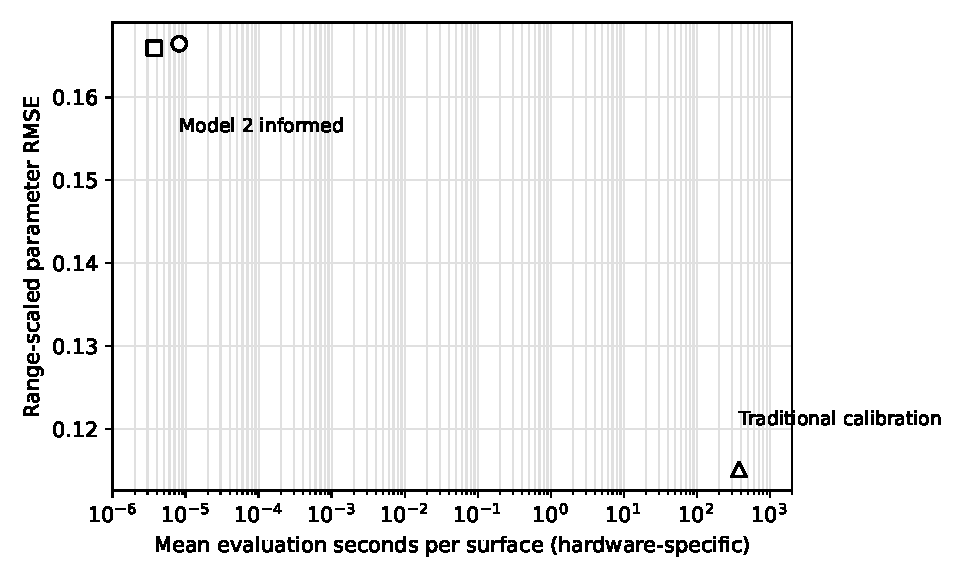
\includegraphics[width=0.78\linewidth]{speed_accuracy_tradeoff.pdf}
\caption{Speed/accuracy position of each method on the untouched synthetic test split.
Runtime axes are hardware-specific provenance.}
\label{fig:speed-accuracy}
\end{figure}

\subsection{Pricing fit does not certify parameters}
Traditional calibration reprices within $10^{-4}$ on 100\% of test surfaces, yet only
$71.92\%$ also have range-scaled parameter RMSE $\leq0.10$ and $94.00\%$ have RMSE
$\leq0.25$. Among neural predictions with repricing nRMSE $\leq10^{-3}$, only about
$7.6\%$ additionally satisfy parameter RMSE $\leq0.10$, although roughly $95\%$ remain
within the looser 0.25 threshold. Figure~\ref{fig:fit-not-recovery} shows why the two
metrics must remain separate.

\begin{figure}[htbp]
\centering
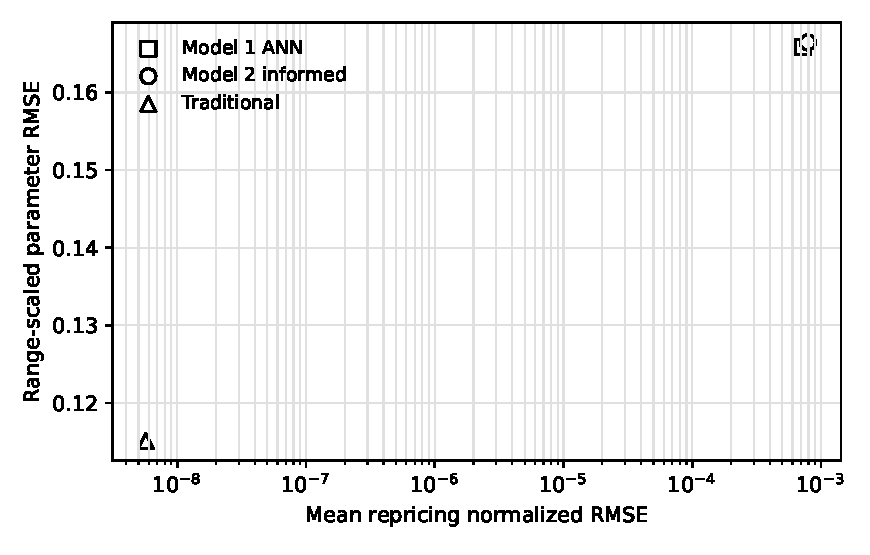
\includegraphics[width=0.70\linewidth]{fit_is_not_recovery.pdf}
\caption{Mean repricing error versus known-truth parameter error. Distance along the
repricing axis does not determine distance along the recovery axis.}
\label{fig:fit-not-recovery}
\end{figure}

\subsection{Stability}
Neural headline metrics are stable across seeds, but per-surface prediction dispersion
is larger for Model2 than Model1; adding differentiable repricing did not reduce seed
dispersion in the completed primary evidence. Traditional multi-start behavior is much
more dispersed: the per-surface start-disagreement rate is $89.16\%$, and 3{,}192 of
3{,}750 starts reach the frozen function-evaluation cap.

\subsection{Observation-noise status}
Table~\ref{tab:completed-neural-noise} and Figure~\ref{fig:neural-noise} report only
the completed neural full-population evaluations. They do not imply that the three-way
positive-noise comparison is finished. Positive-level traditional subset calibration
remains active/pending, so no three-way noise conclusion is drawn here.

\begin{table}[htbp]
\centering
\caption{Completed neural full-test-population observation-noise evaluations.}
\label{tab:completed-neural-noise}
\begin{tabular}{lccccc}
\toprule
Noise & M1 parameter RMSE & M1 clean-latent nRMSE & M2 parameter RMSE & M2 clean-latent nRMSE & Mean recovery $\leq0.25$ \\
\midrule
0\% & 0.165991 & 0.000789 & 0.166914 & 0.001027 & 91.00\% \\
0.10\% & 0.165992 & 0.000789 & 0.166915 & 0.001027 & 91.00\% \\
0.25\% & 0.16599 & 0.000789 & 0.166913 & 0.001027 & 90.99\% \\
0.50\% & 0.166 & 0.000791 & 0.166923 & 0.001029 & 91.00\% \\
1.00\% & 0.166028 & 0.000797 & 0.166948 & 0.001033 & 90.99\% \\
\bottomrule
\end{tabular}
\par\vspace{0.35em}
\begin{minipage}{0.94\linewidth}\small Seed-mean values over seeds 11, 22, and 33 for all 1,250 test surfaces at each level, read from pinned commit e58b36d1ff6c. Positive-level traditional subset completion remains pending and is excluded here.\end{minipage}
\end{table}


\begin{figure}[htbp]
\centering
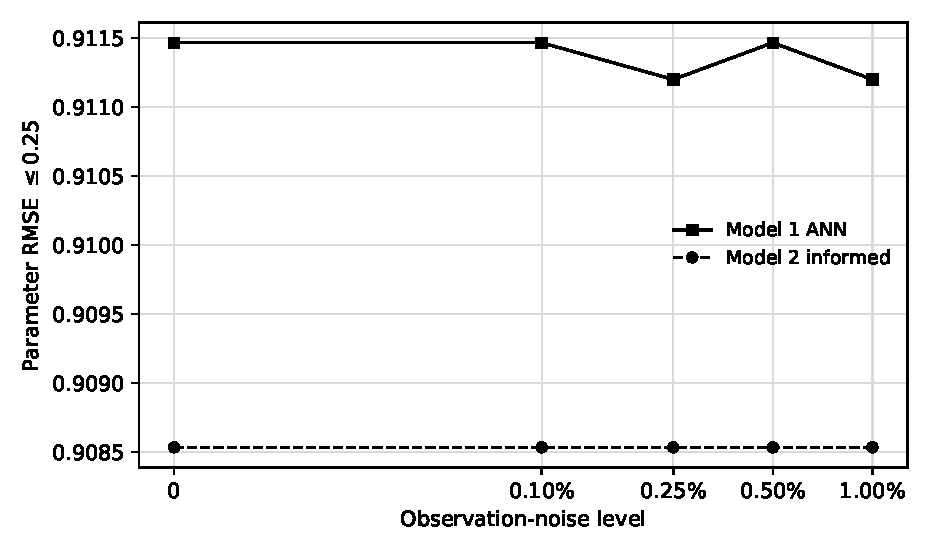
\includegraphics[width=0.76\linewidth]{completed_neural_noise.pdf}
\caption{Completed seed-mean neural recovery rates across observation-noise levels.
Traditional positive-noise results are omitted because they are incomplete.}
\label{fig:neural-noise}
\end{figure}

\section{Identifiability Discussion}
\label{sec:identifiability}

The completed evidence supports practical non-identifiability, not a claim of global
mathematical non-identifiability over all parameter space. Three independent lines are
relevant.

\paragraph{Development diagnostics.}
Earlier market-supported G2 studies found full algebraic rank in many cases while
failing target-blind recovery under clean and noisy observations. A bounded four-case
global study produced 40 clean near-equivalent solutions forming 39 complete-linkage
clusters; median repricing RMSE was $4.708\times10^{-8}$ while median range-scaled
parameter RMSE was 0.1485. These are historical diagnostics relative to R2, but they
motivate the retained finding.

\paragraph{Representation selection.}
R3 improved local conditioning and clean best-start recovery, yet lost under the frozen
realistic-noise rule. At the primary 0.5\% level, selected-R2 best-start displacement
was approximately 0.383 range-scaled RMSE while fitted-surface error was about 0.884\%
relative RMSE. The third expiry adds clean information but does not resolve ambiguity
at observation scale.

\paragraph{Known-truth benchmark.}
On the final synthetic test split, traditional calibration achieves essentially exact
repricing on every surface; $94.00\%$ have range-scaled parameter RMSE $\leq0.25$, so
$6.00\%$ remain above that coarse threshold. This lower-bounds rather than exhausts the
ambiguity problem.

Compensated directions are visible in aggregate metrics. Total initial variance
$v^s_0+v^f_0$ and total long-run variance $\theta_s+\theta_f$ are estimated much better
than individual factors, while kappa or half-life parameters remain difficult for all
methods. Canonical slow/fast ordering is a declared tie-breaker, not evidence that an
unordered factor swap is economically identified.

The correct scientific statement is therefore:
\begin{center}
\texttt{PRACTICAL\_NON\_IDENTIFIABILITY = RETAINED\_RESEARCH\_FINDING}.
\end{center}

\section{Limitations}
\label{sec:limitations}

\subsection{Scope limitations}
The primary benchmark is synthetic with complete surfaces and zero observation noise.
It establishes controlled method behavior under known truth, not real-market profit,
forecasting skill, or universal pricing correctness. The real NTPC pilot is one stock,
one valuation date, short-dated development data, and a small active-quote domain.

\subsection{Protocol limitations}
Traditional calibration receives a disclosed truth-informed start by frozen design.
Its runtime comes from one recorded environment and cannot be compared to neural
training environments as model quality. Model2 uses a single frozen loss configuration;
its repricing weight was not tuned. Neural hardware cohorts differ across Model1 and
Model2 and are provenance only.

\subsection{Identifiers and inference limitations}
Range-scaled and standardized summaries do not replace per-parameter distributions.
Constraint validity means structural legality, not economic truth. Factor ordering is a
declared convention. No posterior, confidence interval, or unique-recovery claim is made.

\section{Pending Experiments}
\label{sec:pending-experiments}

Table~\ref{tab:result-status} separates current completed evidence from work that must
not be inferred from this draft.

\begin{table}[htbp]
\centering
\caption{Result status at the August 25, 2026 synthesis boundary.}
\label{tab:result-status}
\begin{tabular}{p{0.31\linewidth}p{0.20\linewidth}p{0.34\linewidth}}
\toprule
Item & Status & Boundary \\
\midrule
Canonical engine validation & Complete & Controlled implementation evidence only \\
Frozen R2 representation & Complete & Practical non-identifiability retained \\
Final 10k known-truth dataset & Complete & Synthetic engineering conditioning \\
Primary Traditional/ANN/Model2 test & Complete & One frozen synthetic-test evaluation \\
Neural noise through 1\% & Complete & Full neural population only \\
Positive-noise traditional subset & Pending & Required before three-way noise claims \\
OOD/boundary robustness & Not done & Separate protocol required \\
G8 real-market evaluation & Not started & Development dates remain excluded \\
Model3 PDE training & Protocol only & Stage A/B results do not exist \\
\bottomrule
\end{tabular}
\end{table}

\pending{No positive-noise traditional completion is claimed.} The pinned handoff
records a preserved interrupted 0.10\% journal and explicitly states that no final CSV
exists at that level.

\pending{No OOD result is claimed.} Existing boundary/challenge sampling audits are
development readiness evidence, not completed final OOD robustness.

\pending{No G8 result is claimed.} All five NTPC dates used so far are development/
diagnostic dates and are excluded from final real-market evaluation.

\pending{No Model3 result is claimed.} Only the frozen protocol and foundation tests
exist; neither pilot nor research-run outcomes exist here.

\section{Conclusion Draft}
\label{sec:conclusion}

This synthesis organizes completed Double Heston inverse-calibration evidence around a
single defensible message: a validated forward engine and a frozen known-truth dataset
make it possible to compare fast learned inverses against a strong traditional frontier
without conflating speed, structural validity, repricing fit, and parameter recovery.

Under that discipline, traditional numerical calibration remains the accuracy reference
but is computationally expensive. Ordinary ANN and constraint/repricing-informed neural
mappings are dramatically faster and structurally valid, with moderate aggregate errors
and excellent seed stability, but materially larger known-truth errors. Their similar
performance indicates that the differentiable repricing term did not solve the central
inverse problem in the frozen configuration.

The most important conclusion is negative and constructive: low repricing error can
coexist with material parameter displacement. Any useful calibration methodology should
therefore report tolerance-conditioned parameter recovery separately from fit-to-
observations, retain failed starts, disclose constraints and starts, and avoid claiming
unique identification from optimizer success.

The next evidentiary steps are already bounded: finish positive-noise traditional subset
calibration under its frozen protocol, evaluate genuine PDE-informed Model3 only after
the frozen Stage A/B sequence, and reserve OOD and final real-market conclusions for their
separately authorized experiments. Until then, the canonical claim is a frozen
representation plus retained practical non-identifiability, not a solved inverse problem.

\bibliographystyle{plainnat}
\bibliography{references}
\appendix
\section{Appendix Structure and Reproducibility}
\label{app:provenance}

\subsection{Artifact map}
\begin{table}[htbp]
\centering
\caption{Central classification of manuscript evidence at the synthesis boundary.}
\label{tab:evidence-classification}
\begin{tabular}{p{0.20\linewidth}p{0.13\linewidth}p{0.08\linewidth}p{0.27\linewidth}p{0.19\linewidth}}
\toprule
Item & Classification & Commit & Artifact & Boundary \\
\midrule
Canonical engine validation & Canonical & 72ad8e1aa845 & \texttt{outputs/double\_heston\_benchmark/benchmark\_summary.json} & Independent adaptive-quadrature agreement \\
Development NTPC model pilot & Development & 72ad8e1aa845 & \texttt{docs/evidence/NTPC\_SINGLE\_STOCK\_PILOT\_MANIFEST.json} & NO\_CLEAR\_WINNER \\
Frozen R2 representation & Canonical & 72ad8e1aa845 & \texttt{docs/R2\_REPRESENTATION\_CONTRACT.md} & Selected by sealed R2/R3 rule \\
Final 10k synthetic dataset & Canonical & b13caf0747d3 & \texttt{data/final\_r2\_clean\_10000/manifest.json} & Full replay: VERIFIED\_IDENTICAL\_FULL\_REPLAY \\
Primary method comparison & Canonical & 72ad8e1aa845 & \texttt{evidence/r2\_primary\_comparison\_20260823/FINAL\_EVALUATION\_EVIDENCE\_MANIFEST.json} & First test read: true \\
Neural positive-noise evaluations & Complete subset of noise protocol & e58b36d1ff6c & \texttt{origin/codex/r2-noise-recovery:evidence/r2\_noise\_robustness/neural/MANIFEST.json} & Full neural population; traditional positives pending \\
Positive-noise traditional calibration & Active/pending & e58b36d1ff6c & \texttt{origin/codex/r2-noise-recovery:docs/R2\_NOISE\_CLOUD\_EXECUTION\_HANDOFF.md} & No positive-level final CSV exists \\
Model3 PDE methodology & Frozen protocol only & 02c2a2cbc249 & \texttt{origin/research/model3-pde-protocol:docs/MODEL3\_PDE\_PROTOCOL.md} & No Model3 training result exists \\
Pre-R2 G2 diagnostics and 108 grid & Superseded/historical & 72ad8e1aa845 & \texttt{docs/RESULTS\_TO\_DATE.md}; \texttt{docs/G2\_R2\_R3...} & Motivation and method development only \\
Model2 local CPU seed-11 replication & Non-primary execution replica & 72ad8e1aa845 & \texttt{evidence/r2\_primary\_comparison\_20260823/training\_run\_manifest.json} & Excluded from primary cohort \\
\bottomrule
\end{tabular}
\par\vspace{0.35em}
\begin{minipage}{0.94\linewidth}\small The complete claim-to-artifact mapping is maintained in \texttt{paper/RESULTS\_INVENTORY.md}; this appendix table is a compact audit view.\end{minipage}
\end{table}


\subsection{Reproducibility commands}
\begin{verbatim}
C:\Python313\python.exe paper\scripts\generate_results_assets.py
C:\Python313\python.exe paper\scripts\validate_paper.py
git show e58b36d1ff6cbf39115d46698ad0fb45b1ac1b8b:evidence/r2_noise_robustness/neural/all_neural_seed_headline.csv
\end{verbatim}

\subsection{Environment and validation record}
Asset generation used Python 3.13.4, pandas 2.3.2, and matplotlib 3.10.6 on the audit
host. PDF compilation could not be run because no LaTeX executable was installed there;
\texttt{pdflatex}, \texttt{latexmk}, and Tectonic were absent. Structural validation
covers required sections, generated assets, inventory coverage, balanced common LaTeX
environments, pinned commits, placeholder-only citations, and ASCII source/output.

\subsection{Future appendix placeholders}
\placeholder{Detailed metric definitions.} Insert exact formulas from the frozen
evaluation module after final writing review.

\placeholder{Per-seed and per-parameter tables.} Add only after selecting tables from
the immutable evidence bundle; do not recompute experiments.

\placeholder{Data-selection audit.} Summarize official-source hashes and exclusions
without printing confidential row-level data.

\placeholder{Model3 pre-registration excerpt.} Quote the frozen protocol commit and
config hash when the experiment becomes active.


\end{document}
